\newpage
\section{Oppbygging av programmet}
\thispagestyle{fancy}

\subsection{Programmeringsmetode}
For å sette i sammen alle funksjonsblokkene, som vi hadde skreve i strukturert tekst, valgte vi å bruke \GLS{Codesys} CFC.
CFC (Continuous Function Chart) er er ein grafisk programmeringsmetode som bruker symbol og koplingar for å gjere programmet  meir visuelt.

Alle sammensettningar av blokker valgte vi å gjere i CFC. Ved å bruke ein grafisk metode sikra vi oss god lesbarhet og
visuell forståelse i programmet. 

Alle inngangar og utgangar er leselige og enkle og forstå. CFC ilag med god dokumentasjon vil kunne gi personar utan programmeringsbakgrunn
god forståelse av korleis programmet er satt opp, utan å måtte lese linjer med kode.
CFC gir godt grunnlag for feilsøking og analyse og bygger derfor vidare på filosofien med eit enkel og fleksibelt program.

Dersom antall koplingar og linjer gjorde programmet vanskeleg å lese var det også
mogleg å opprette `source' og `links' som oppretta ein trådlaus forbindelsane gjennom ein unik ID.


\begin{figure}[htbp]
    \centering
    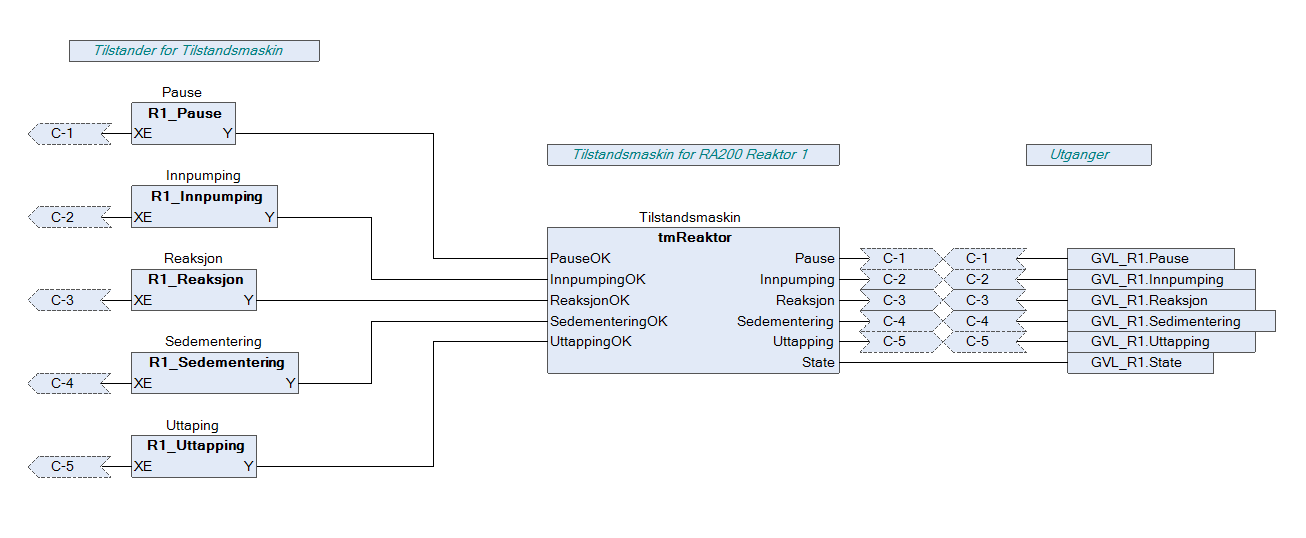
\includegraphics[width=1\textwidth]{Bilder/ReaktorPRG.png}
    \caption{Eksempel CFC - Styring reaktor 1}\label{fig:reaktorsoner}
\end{figure}

\newpage

\subsection{Hovuddel}

Programmet er delt opp i tre hovuddelar, ei tilstandsmaskin for kvar reaktor og ein del for samling av felles reaktor funksjonar.
Alle desse har eit kall i MainTask og blir utført kvar PLS syklus. Tilstandsmaskina har overordna ansvar og bytter på kva 
\gls{FB} med tilstandslogikk som køyrer.

Felles funksjonar er ein samling av funksjonsblokker og utrekningar som er felles og eller uavhengig av reaktorane med tilstandsmaskin.
Driftsovervåking er ein sentral del av felles funksjoner, der timetelling og mengde prosessert vatn er eksempel på funksjonar og utrekningar
som blir gjennomført.

I enkelte tilfeller måtte, som ved rullering av sivbed, var vi avhengig av at både tilstandsmaskin for reaktor 1 og reaktor 2 hadde samme informasjonen.
Dette løyste vi ved å lage ei fbSivbedRotation i felles funsjonar som henter inn og akummulerte antall slamutakk for så å rotere når ei git grense var nådd.
Denne informasjonen blir så sendt til kvar tilstandsmaskin og sørger for at begge reaktorane har same aktive sivbed.


\begin{figure}[htbp]
    \centering
    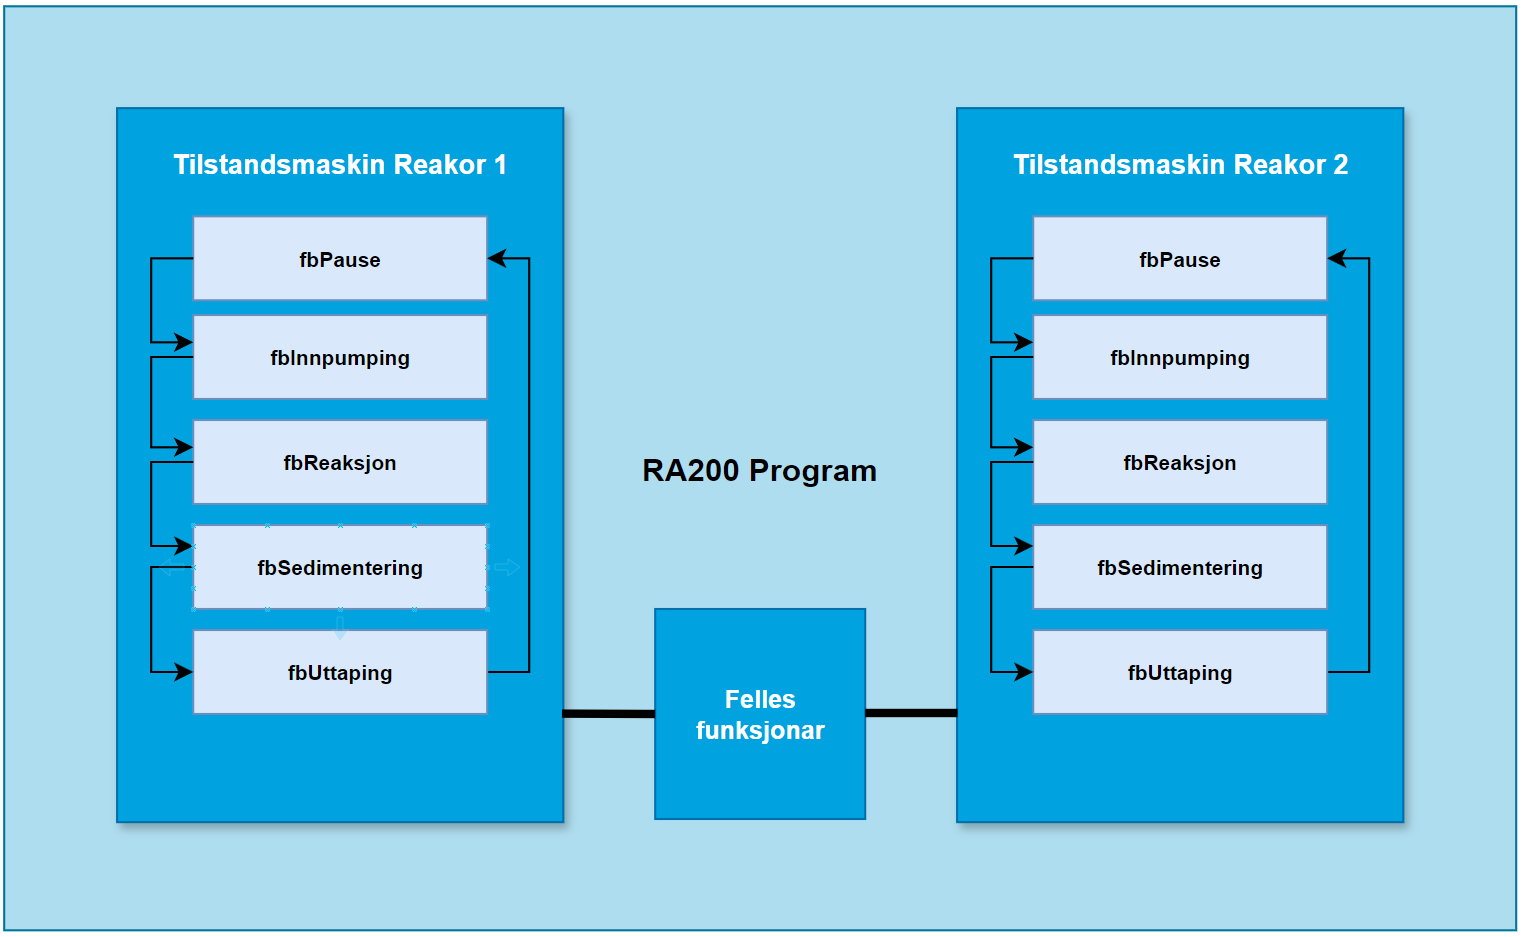
\includegraphics[width=1\textwidth]{Figurar/Oppbygging_Program.png}
    \caption{Illustrasjon oppbygging av programmet}\label{fig:reaktorsoner}
\end{figure}


\newpage

\subsection{Styring tilstandslogikk}

Som nemnt tilegare er det tilstandslogikken som samarbeider opp mot IEC blokkene. Dette samarbeidet valge vi også å gjere i eit
CFC vindu som igjen gjorde kall og koplingar visuelle. Dette CFC vinduet fikk navn etter kva sekvens i SBR-prosessen
den hadde ansvar for å styre. 

Oppbyggningen av desse sekvensstyringane er gjort med inngangsblokker (MA og MB) øvst og utgangsblokker (SBE og SBV) i bunn.
I mellom desse kjem sjølve tilstandslogikk blokkene som inneholder sjølve logikken.

\begin{figure}[htbp]
    \centering
    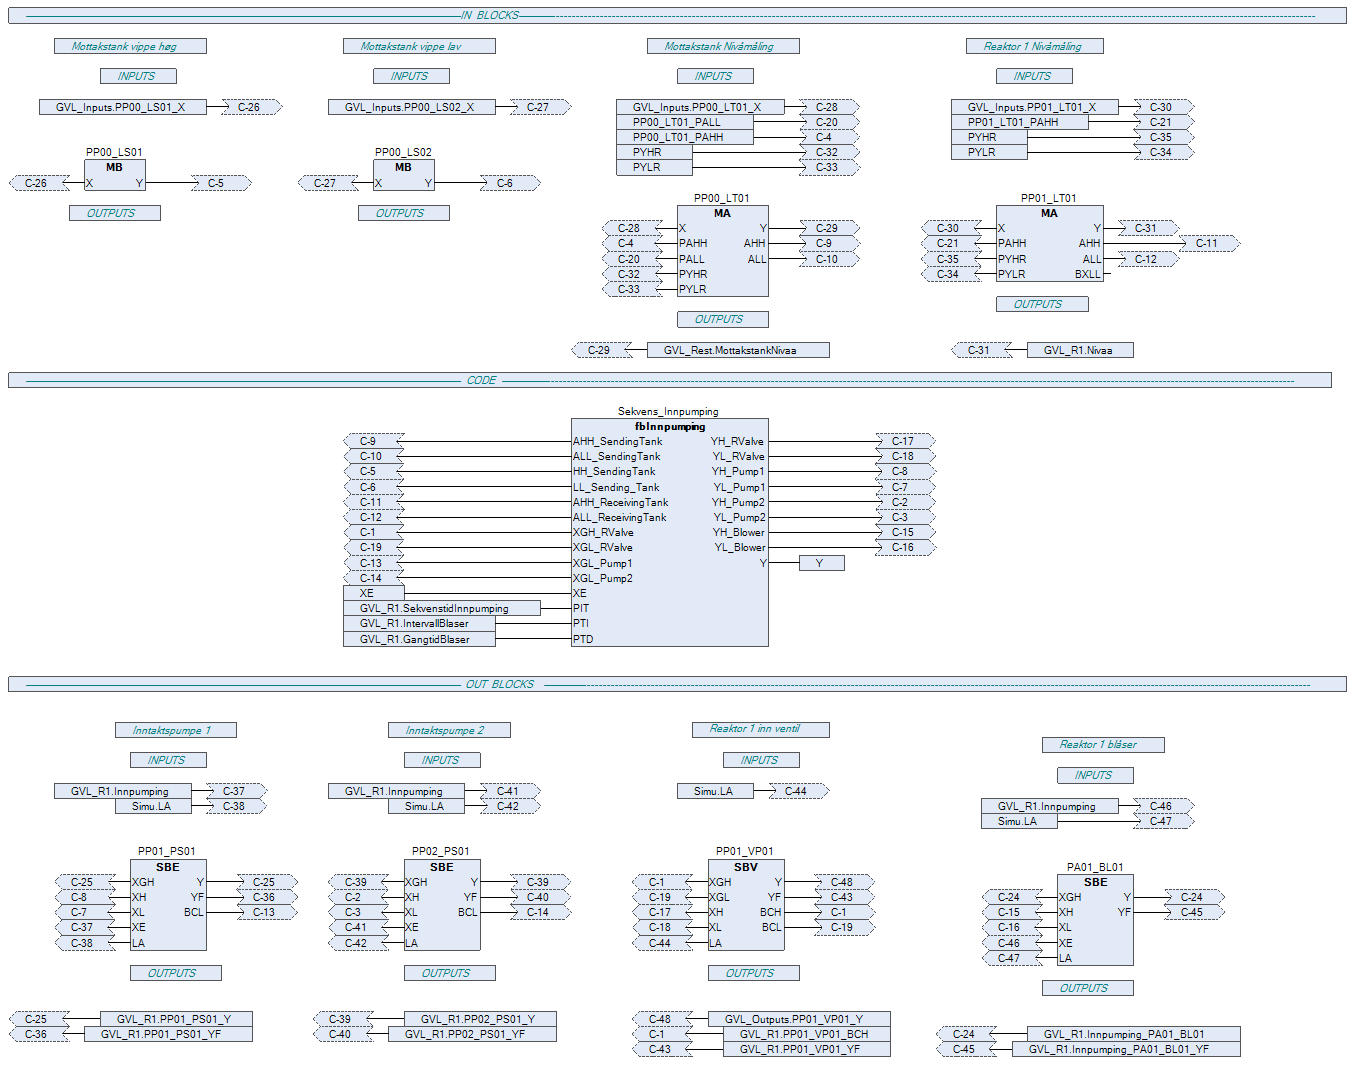
\includegraphics[width=1\textwidth]{Bilder/Heile_innpump.png}
    \caption{Eksempel CFC - Styring Innpumping}\label{fig:reaktorsoner}
\end{figure}

I denne figuren er ekstra inngangar, parameter inngangar og ekstra utgangar fjerna for å bedre visualisere kopllinga og samarbeidet mellom
IEC blokkene og funksjonsblokk for tilstandslogikk.

\newpage

